\documentclass{article}
\usepackage[usenames, dvipsnames]{color}
\usepackage{fancyhdr}
\usepackage{extramarks}
\usepackage{amsmath}
\usepackage{amssymb}
\usepackage{mathtools}
\usepackage{amsthm}
\usepackage{amsfonts}
\usepackage[per-mode=fraction]{siunitx}
\usepackage{tikz}
\usepackage{graphicx}
\usepackage{float}
\usepackage{afterpage}
\usepackage{systeme}
\usepackage{makecell}
\usepackage{nicematrix}
\usepackage{physics}
\usepackage{float}
\usepackage{tikz}
\usetikzlibrary{math,arrows,positioning,shapes,fit,calc}
\usepackage{dsfont}
\usepackage{wrapfig}
\usepackage{pgfplots}
\usepackage{esint}
\pgfplotsset{compat=1.8}

\definecolor{mediumgreen}{RGB}{0,153,0}
\newtheorem{theorem}{Theorem}[section]
\newtheorem{lemma}[theorem]{Lemma}
\usetikzlibrary{trees}

%
% Basic Document Settings
%

\topmargin=-0.45in
\evensidemargin=0in
\oddsidemargin=0in
\textwidth=6.5in
\textheight=9.0in
\headsep=0.25in

\linespread{1.1}

\pagestyle{fancy}
\lhead{}
\chead{\hmwkClass\ (\hmwkClassInstructor\/): \hmwkTitle}
\rhead{\firstxmark}
\lfoot{\lastxmark}
\cfoot{\thepage}

\renewcommand\headrulewidth{0.4pt}
\renewcommand\footrulewidth{0.4pt}

\setlength\parindent{0pt}

%
% Create Problem Sections
%

\newcommand{\enterProblemHeader}[1]{
    \nobreak\extramarks{}{Problem \arabic{#1} continued on next page\ldots}\nobreak{}
    \nobreak\extramarks{Problem \arabic{#1} (continued)}{Problem \arabic{#1} continued on next page\ldots}\nobreak{}
}

\newcommand{\exitProblemHeader}[1]{
    \nobreak\extramarks{Problem \arabic{#1} (continued)}{Problem \arabic{#1} continued on next page\ldots}\nobreak{}
    \stepcounter{#1}
    \nobreak\extramarks{Problem \arabic{#1}}{}\nobreak{}
}

\setcounter{secnumdepth}{0}
\newcounter{partCounter}
\newcounter{homeworkProblemCounter}
\setcounter{homeworkProblemCounter}{1}
\nobreak\extramarks{Problem \arabic{homeworkProblemCounter}}{}\nobreak{}

%
% Homework Problem Environment
%
% This environment takes an optional argument. When given, it will adjust the
% problem counter. This is useful for when the problems given for your
% assignment aren't sequential. See the last 3 problems of this template for an
% example.
%
\newenvironment{homeworkProblem}[1][-1]{
    \ifnum#1>0
        \setcounter{homeworkProblemCounter}{#1}
    \fi
    \section{Problem \arabic{homeworkProblemCounter}}
    \setcounter{partCounter}{1}
    \enterProblemHeader{homeworkProblemCounter}
}{
    \exitProblemHeader{homeworkProblemCounter}
}

%
% Homework Details
%   - Title
%   - Due date
%   - Class
%   - Section/Time
%   - Instructor
%   - Author
%

\newcommand{\hmwkTitle}{Homework 2}
\newcommand{\hmwkDueDate}{Sunday January 16, 2022}
\newcommand{\hmwkClass}{Math 382}
\newcommand{\hmwkClassTime}{Section A}
\newcommand{\hmwkClassInstructor}{Prof. Ezra Getzler}
\newcommand{\hmwkAuthorName}{\textbf{Anthony Tam}}

%
% Title Page
%

\title{
    \vspace{2in}
    \textmd{\textbf{\hmwkClass:\ \hmwkTitle}}\\
    \normalsize\vspace{0.1in}\small{Due\ on\ \hmwkDueDate\ at 5:00 PM}\\
    \vspace{0.1in}\large{\textit{\hmwkClassInstructor\ }}
    \vspace{3in}
}

\author{\hmwkAuthorName}
\date{}

\renewcommand{\part}[1]{\textbf{\large Part \Alph{partCounter}}\stepcounter{partCounter}\\}

%
% Various Helper Commands
%

% For derivatives
\newcommand{\deriv}[1]{\frac{\mathrm{d}}{\mathrm{d}x} (#1)}

% For partial derivatives
\newcommand{\pderiv}[2]{\frac{\partial}{\partial #1} (#2)}

% Integral dx
\newcommand{\dx}{\mathrm{d}x}

% Alias for the Solution section header
\newcommand{\solution}{\textbf{\large Solution}}

% Probability commands: Expectation, Variance, Covariance, Bias
\newcommand{\E}{\mathrm{E}}
\newcommand{\Var}{\mathrm{Var}}
\newcommand{\Cov}{\mathrm{Cov}}
\newcommand{\Bias}{\mathrm{Bias}}

\newcommand*\circled[1]{\tikz[baseline=(char.base)]{
            \node[shape=circle,draw,inner sep=2pt] (char) {#1};}}

\newcommand\myeqq{\stackrel{\mathclap{\normalfont\mbox{\scriptsize\text{set}}}}{=}}

\makeatother

\begin{document}

\maketitle

\pagebreak

\begin{homeworkProblem}
  Consider the annulus $U=\{z \in \mathbb{C}|a<| z \mid<b\}$, where $0<a<b<\infty$. Show that $U$ is a domain.
In showing that any two points of $U$ may be joined by a path, you may exhibit a path that is piecewise differentiable. The original question was to show that you may choose the path to be piecewise linear; if you can do that, you may derive satisfaction for a job well done.\\

\solution\\

\vspace{-0.5cm}

\begin{proof}

To show that $U$ is a domain, we need to \textcircled{\tiny{1}} show that $U \subseteq \mathbb{C}$ is open and \textcircled{\tiny{2}} show that $U$ is path connected. For \textcircled{\tiny{1}}, define the sets
\begin{align*}
 S_1 = \left\{ z \in \mathbb{C} \, \middle| \, \abs{z} > a \right\} \;\text{ and }\; S_2 = \left\{ z \in \mathbb{C} \, \middle| \, \abs{z} < b \right\}
 .\end{align*}
We claim that both $S_1$ and $S_2$ are open. For $S_1$, recall that any set is open if and only if its complement is closed. Thus, consider $S_1^C = \left\{ z \in \mathbb{C} \,\middle|\, \abs{z} \leq a \right\}$, a closed ball of radius $a$. But note that the boundary $\partial S_1^C = \left\{ z \in \mathbb{C} \, \middle| \, \abs{z} = a \right\} \subset S_1^C$, i.e., $S_1^C$ contains its boundary so the complement is closed and $S_1$ is open. For $S_1$ note that the region is simply an open ball of radius $b < \infty$, so is open by the result shown in class. Now observe the intersection of these two sets is exactly $S_1 \cap S_1 = U$ and the intersection of two open sets is itself open, so in particular $U$ is open. For \textcircled{\tiny{2}}, we need to show that $U$ is path connected. Let $z_1, z_2 \in U$. Then write both in polar form:
\begin{align*}
 z_1 = r_1 e^{i \theta_1} \; \text{ and } \; z_2 = r_2 e^{i\theta_2}
 .\end{align*}
Note that since $z_1, z_2 \in U$, we must have $a < r_1, r_2 < b$. Now we claim that the choice of the two following paths, namely
\begin{align*}
 \gamma(t) = r_1 e^{i (\theta_1 + t(\theta_2 - \theta_1))} \; \text{ and } \; \xi(t) = (r_1 + t(r_2 - r_1))e^{i \theta_2}
 \end{align*}
both for $t \in [0, 1]$, give a piecewise differentiable path $\gamma \cup \xi$ that connects $z_1$ and $z_2$. First note that the exponential function and affine function are certainly differentiable, so respectively $\gamma$ and $\xi$ are differentiable functions of $t$ and their concatentaion is then also piecewise differentiable. Then note that geometrically, $\gamma$ starts at $z_1$ and traverses along the circle of radius $r_1$ centered at the origin in a CCW fashion as $t$ runs from $0 \to 1$. When $t = 1$, $\gamma$ ends at $\gamma(1) = r_1e^{i \theta_2}$, which is radial with $z_2$. Then the concatenation with $\xi$ traverses in a straight line along the radial direction until it hits $z_2$ as $t$ runs from $0 \to 1$, upon which $\xi(1) = r_2 e^{i\theta_2} = z_2,$ as claimed. Thus, $U$ is open and path connected, i.e., it is a domain.

\begin{figure}[H]
  \centering
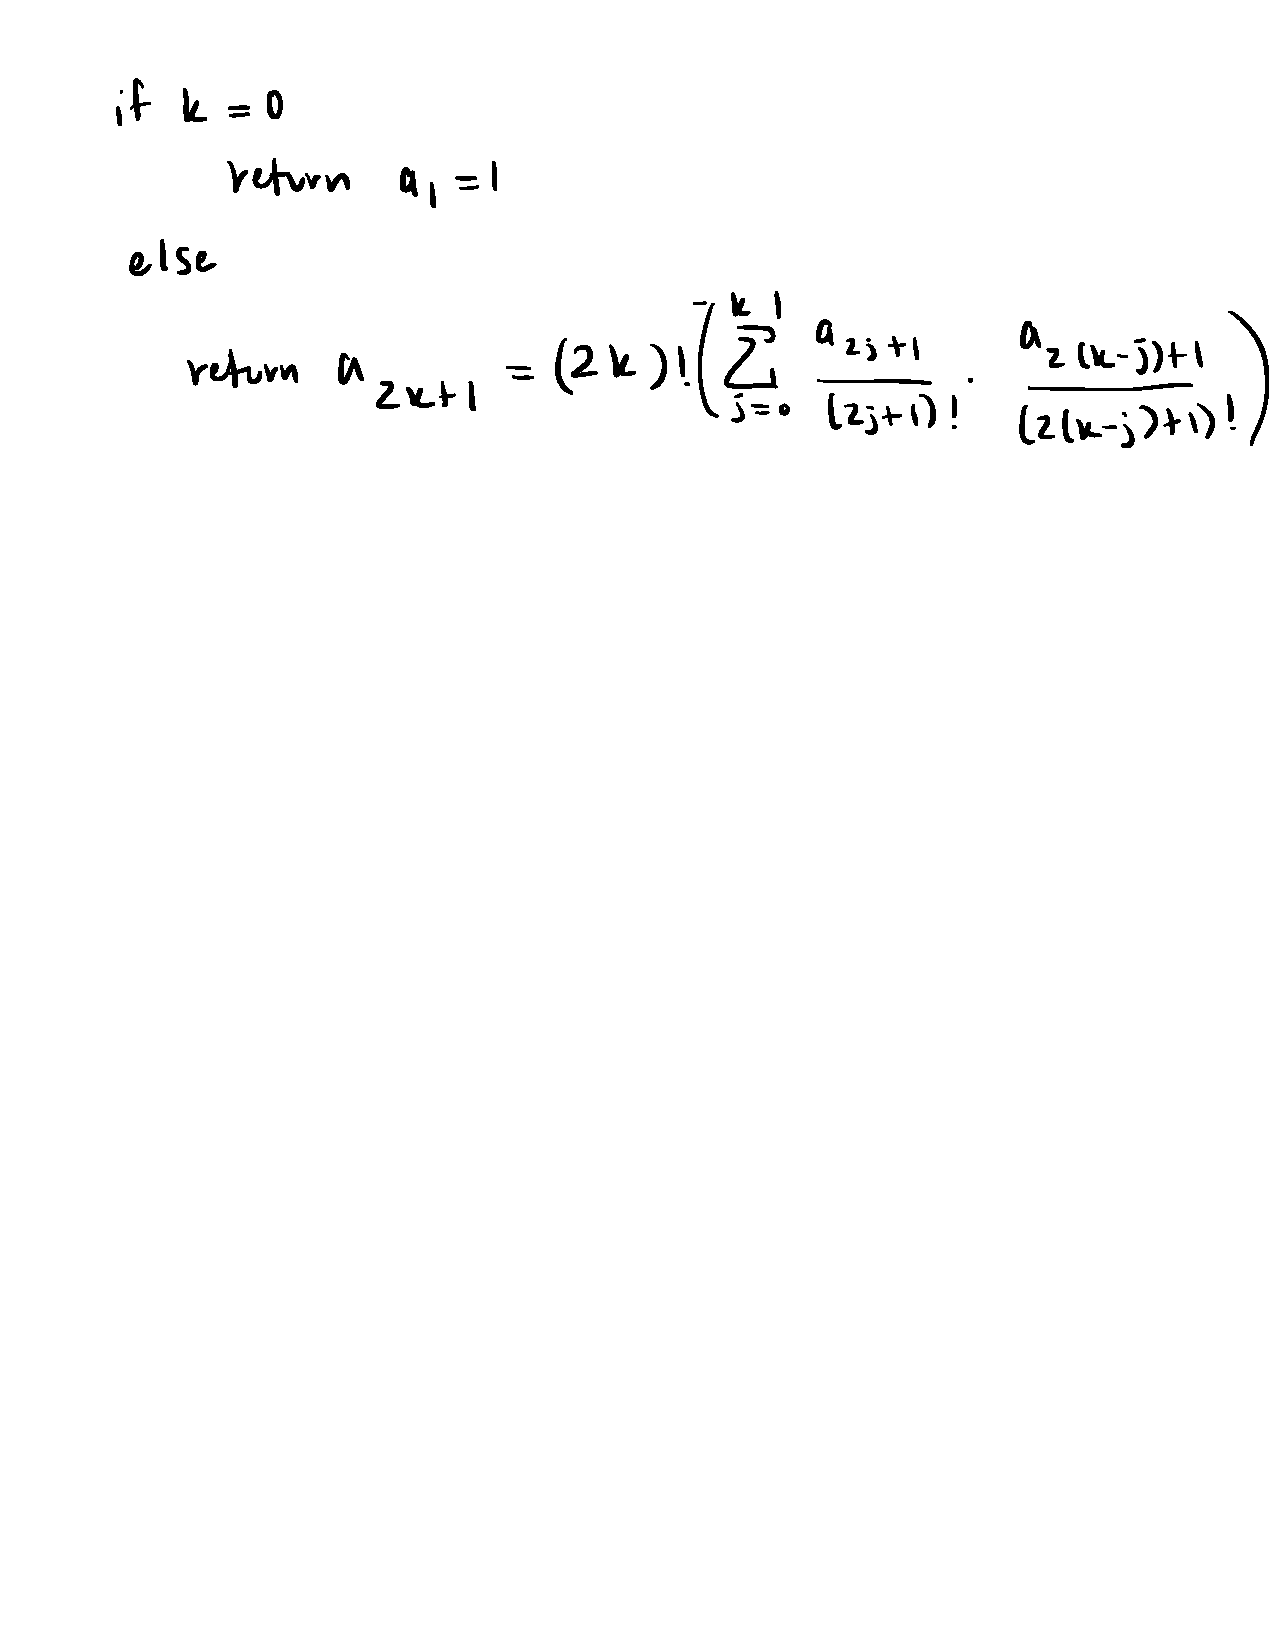
\includegraphics[trim = 2cm 20cm 2cm 1.5cm, clip]{figure}
\caption{Two paths that connect $z_1$ and $z_2$ in $U.$}
\end{figure}

For the challenge, another way to see that $U$ is path connected but \textit{only} using a \textit{polygonal} path is to draw an open ball centered at $z_1$ of radius $b-a$ contained in $U$, i.e, $B_1(b-a, z_1) \subset U$, and now draw any radial line from the center to the edge of the ball in the direction of $z_2$. This line, call it $\ell_1$, is indeed a path since the ball is convex. Then draw another ball $B_2(b-a, w_1)$ where $w$ lies on the circle of radius $r_1$ centered at the origin, i.e., $w_1$ and $z$ lie on the same circle centered at the origin. Now you can draw \textit{any} line $\ell_2$ that starts from the end of $\ell_1$ in the direction of $z_2$ until you hit the edge of the ball, and by convexity of the ball $\ell_2$ is still a path contained in the ball. Continue this process until the ball $B_i(b-a, w_i)$ contains the point $z_2$, upon which you can always draw a straight line from the edge of the ball where $\ell_{i-1}$ stopped to the point $z_2$ since the open ball is path connected. The union of all the paths $\gamma = \ell_1 \cup \ell_2 \cdots \ell_i$ gives a polygonal path from $z_1$ to $z_2$ and thus $U$ is path connected.
\end{proof}

\end{homeworkProblem}

\pagebreak

\begin{homeworkProblem}
  Verify by calculating the partial derivatives with respect to $x$ and $y$, the real and imaginary parts of $z$, that the function $\sin (z)$ satisfies the Cauchy-Riemann equation.\\

  \solution\\

  First write $f(z) = \sin{z}$ in complex exponential form:
  \begin{align*}
   \sin{z} = \frac{e^{iz} - e^{-iz}}{2i}
  \end{align*}
  Then writing the complex number $z$ as $z = x + iy$ for $x, y \in \mathbb{R}$, we can expand and simplfify the sine as
  \begin{align*}
    \sin{z} &= \frac{e^{i(x+iy)} - e^{-i(x + iy)}}{2i}\\
    &= \frac{e^{ix}e^{-y} - e^{-ix}e^y}{2i}\\
    &= \frac{(\cos{x} + i \sin{x})e^{-y}}{2i} - \frac{(\cos{x} - i\sin{x})e^y}{2i}\\
    &= \cos{x} \frac{e^{-y}}{2i} + \sin{x} \frac{e^{-y}}{2} - \cos{x} \frac{e^y}{2i} + \sin{x} \frac{e^y}{2}\\
    &= \cos{x} \left( \frac{e^{-y} - e^y}{2i} \right) + \sin{x} \left( \frac{e^y + e^{-y}}{2}\right)\\
    &= \sin{x} \left( \frac{e^y + e^{-y}}{2} \right) + i \cos{x} \left( \frac{e^y - e^{-y}}{2} \right)\\
    &= \sin{x} \cosh{y} + i\cos{x} \sinh{y}
   ,\end{align*}
  where we used the identity $e^{ix} = \cos{x} + i \sin{x}$. Now let $u = \sin{x} \cosh{y}$ and $v = \cos{x}\sinh{y}$ so that
  \begin{align*}
   f(z) = u + iv
   .\end{align*}
  Then we can compute
  \begin{alignat*}{2}
   \frac{\partial u}{\partial x} &= \cos{x}\cosh{y} \hspace{0.5cm} &&\frac{\partial u}{\partial y} = \sin{x}\sinh{y}\\
   \frac{\partial v}{\partial y} &= \cos{x}\cosh{y} \hspace{0.5cm} &&\frac{\partial v}{\partial x} = -\sin{x}\sinh{y}
   .\end{alignat*}
  So, we have
  \begin{align*}
    \frac{\partial u}{\partial x} = \frac{\partial v}{\partial y} \; \text{ and } \; \frac{\partial u}{\partial y} = -\frac{\partial v}{\partial x}
   ,\end{align*}
  so $f(z) = \sin{z}$ satisfies the Cauchy-Riemann equations.
\end{homeworkProblem}

\pagebreak

\begin{homeworkProblem}
  Consider the square with vertices $\{0,1,1+i, i\}$. Let $\gamma$ be a parametrized path that follows the four sides of this square in a counterclockwise direction.

  a) If $g(x, y) d x+h(x, y) d y$ is a differential defined on an open set containing the square, calculate the line integral
  $$
  \int_{\Gamma} g(x, y) d x+h(x, y) d y
  $$
  in terms of explicit definite integrals.

  b) Calculate this line integral for the differentials $d z, z d z$ and $z^{2} d z$. Do you see a pattern?

  c) Calculate the line integral for the differential $\bar{z} d z$.\\

  \solution\\

  \part\\

We first parametrize the unit square with vertices $\{0,1,1+i, i\}$ in a CCW fashion: let $\Gamma$ be the concatentation of piecewise line segments $C_1$, $C_2$, $C_3$, and $C_4$, each parametrized respectively by
\begin{align*}
 \begin{cases}
  \gamma_1(t) = t + 0 i, & t \in [0,1]\\
  \gamma_2(t) = 1 + ti, & t \in [0,1]\\
  \gamma_3(t) = (1-t) + i, & t \in [0,1]\\
  \gamma_4(t) = 0 + (1-t)i, & t \in [0,1],
 \end{cases}
 \end{align*}
such that $\Gamma = C_1 \cup C_2 \cup C_3 \cup C_4 $ gives the desired piecewise differentiable parametrization. Then the line integral of the 1-form $g(x,y)dx + h(x,y) dy$ over $\Gamma$ is
\begin{align*}
 \int_{\Gamma}g(x,y)dx + h(x,y) dy &= \int_{C_1}g(x,y)dx + h(x,y) dy + \cdots + \int_{C_4}g(x,y)dx + h(x,y) dy\\
 &= \int_{0}^{1}[g(\gamma_1(t))\gamma_1'(t) + h(\gamma_1(t))\gamma_1'(t)]\;dt + \cdots + \int_{0}^{1}[g(\gamma_4(t))\gamma_4'(t) + h(\gamma_4(t))\gamma_4'(t)]\;dt
 .\end{align*}
Then computing
\begin{align*}
 \gamma_1'(t) = 1, \gamma_2'(t) = i, \gamma_3'(t) = -1,\text{ and } \gamma_4(t) = -i
 \end{align*}
gives us that
\begin{align*}
  \int_{\Gamma}g(x,y)dx + h(x,y) dy = \int_{0}^{1}&[g(\gamma_1(t))+ h(\gamma_1(t))]\;dt + i\int_{0}^{1}[g(\gamma_2(t))+ h(\gamma_2(t))]\;dt\\
  &- \int_{0}^{1}[g(\gamma_3(t))+ h(\gamma_3(t))]\;dt -i\int_{0}^{1}[g(\gamma_4(t))+ h(\gamma_4(t))]\;dt
 .\end{align*}

\part\\

Using the result of \textbf{Part A}, for the differential form $dz$ we have
\begin{align*}
  \int_{\Gamma}g(x,y)dx + h(x,y) dy = \int_{0}^{1}\;dt + i \int_{0}^{1}\;dt - \int_{0}^{1}\;dt - i \int_{0}^{1}\;dt = 0
 .\end{align*}
Similarly, for $zdz$ we have
\begin{align*}
 \int_{\Gamma}g(x,y)dx + h(x,y) dy &= \int_{0}^{1}t\;dt + i \int_{0}^{1}(1+ti)\;dt - \int_{0}^{1}(1-t+i)\;dt - i \int_{0}^{1}(1-t)i\;dt \\
 &= 1 + i - 1 - 1 + 1 - i + 1 - 1 \\
 &= 0
 .\end{align*}
Finally, for $z^2dz$ we have
\begin{align*}
 \int_{\Gamma}g(x,y)dx + h(x,y) dy &= \int_{0}^{1}t^2\;dt + i \int_{0}^{1}(1+ti)^2\;dt - \int_{0}^{1}(1-t+i)^2\;dt - i \int_{0}^{1}((1-t)i)^2\;dt \\
 &= \frac{1}{3} - 1 + \frac{2}{3}i + \frac{2}{3} - i + \frac{1}{3}i\\
 &= 0
 .\end{align*}
 It seems like the line integral along $\Gamma$ for all of these differential forms is zero. This seems to be reflective of the classic multivariable result that if $U \subseteq \mathbb{R}^n$ is open and $\mathbf{F}: U \to \mathbb{R}^n$ is a continuous, conservative vector field on $U$, then the closed line integral vanishes, that is $\oint_C \mathbf{F} \cdot d \mathbf{s} = 0$, for every piecewise oriented closed curve $C$ in $U$. This follows from the existence of a potential function for $\mathbf{F}$ since it is conservative and the fundamental theorem of line intergals.\\

 \part\\

 Using the result of \textbf{Part A}, for $\overline{z}dz$ we have
 \begin{align*}
    \int_{\Gamma}g(x,y)dx + h(x,y) dy &= \int_{0}^{1}t \;dt + i \int_{0}^{1}(1-ti)\;dt - \int_{0}^{1}(1-t-i)\;dt - i \int_{0}^{1}-(1-t)i\;dt\\
    &= 2i
  .\end{align*}
If the observation made in \textbf{Part B} is correct, then this follows from the fact that $\overline{z}$ does not have an antiderivative, whatever that means.
\end{homeworkProblem}

\end{document}
